\chapter{Unitarity and gauge invariance}
In the Heisenberg pictures, where operators are time dependent and states are time independent, we may take two orthonormal bases for the Hilbert, or Fock, space 
\begin{enumerate}
    \item $\ket{\alpha,\ingoing}$ for observation at $t \to \infty$;
    \item $\ket{\alpha,\outgoing}$ for observations at $t \to -\infty$.
\end{enumerate}
The scattering matrix $S$ has elements 
\begin{equation}
    S_{\beta\alpha} = \mybraket{\beta,\outgoing}{\alpha,\ingoing}.
\end{equation}
Since ``in'' states are orthonormal $\mybraket{\alpha,\ingoing}{\beta,\outgoing} = \delta_{\alpha\beta}$, we may insert a complete set of ``out'' states in the relation above to find
\begin{equation}
    \nsum_k\mybraket{\alpha,\ingoing}{k,\outgoing}\mybraket{k,\outgoing}{\beta,\ingoing} = \nsum_k(S_{k\alpha})^\dg S_{k\beta} = \delta_{\alpha\beta},
\end{equation}
or simply $S^\dg S = SS^\dg = \MI$. The optical theorem connects this relation to the fact that the imaginary part of the forward scattering amplitude is related to the cross-section. There is a more general connection to the discontinuities of loop amplitudes. Let $S = \MI + iT$ where $T$ is the transition matrix. Inserting this into $SS^\dg = \MI$ leads to 
\begin{equation}
\label{eq: optical theorem equation}
    -i(T - T^\dg) = TT^\dg = T^\dg T.
\end{equation}
The scattering amplitude $\amp$ from a state $I$ to a state $F$ is defined by
\begin{equation}
\label{eq: generic scattering amplitude}
    \mybrakett{F}{T}{I} = i(2\pi)^4\delta^{(4)}(p_I - p_F)\amp(I \to F),
\end{equation}
where $p_I$ is the total incoming momentum and $p_F$ is the total outgoing one. Combining equations \eqref{eq: optical theorem equation} and \eqref{eq: generic scattering amplitude} gives
\begin{equation}
    -i\mybrakett{F}{T}{I} + i\mybrakett{F}{T^\dg}{I} = \mybrakett{F}{T^\dg T}{I} = \sumint_k \mybrakett{F}{T^\dg}{K}\mybrakett{K}{T}{I},
\end{equation}
where
\begin{equation}
    \sumint_k \equiv \sum_{n=2}^\infty\int\prod_{j=1}^n\frac{d^3k_j}{(2\pi)^32E_j},\quad E_j^2 = |\vk_j|^2 + m_j^2,
\end{equation}
then
\begin{equation}
    \begin{split}
        \mybrakett{F}{T^\dg T}{I} &= \sumint_k[i(2\pi)^4\delta^{(4)}(p_K - p_F)\amp(F \to K)]^\dg \\
        &\times[i(2\pi)^4\delta^{(4)}(p_K - p_I)\amp(I \to K)] \\
        &= \sumint_k(2\pi)^8\delta^{(4)}(p_K - p_F)\delta^{(4)}(p_K - p_I)\amp(F \to K)^\dg\amp(I \to K) \\
        &= \sumint_k(2\pi)^8\delta^{(4)}(p_I - p_F)\delta^{(4)}(p_K - p_I)\amp(F \to K)^\dg\amp(I \to K),
    \end{split}
\end{equation}
hence
\begin{equation}
\label{eq: action difference}
    \amp(I \to F) - \amp(F \to I)^\dg = \sumint_k(2\pi)^4\delta^{(4)}(p_K - p_I)\amp(F \to K)^\dg\amp(I \to K).
\end{equation}
If we set $F = I$ we recover the optical theorem
\begin{equation}
    \begin{split}
        2i\Im{[\amp(I \to I)]} &= \sumint_k(2\pi)^4\delta^{(4)}(p_K - p_I)|\amp(I \to K)|^2 \\
        &= \sum_{k=2}^\infty\int d\Phi_k(p_I;p_1,\dots,p_K)|\amp(I \to K)|^2,
    \end{split}
\end{equation}
where $d\Phi_k(p_I;p_1,\dots,p_K)$ is the $K$-particle phase space integral. We may represent relation \eqref{eq: action difference} graphically by 
\begin{equation}
    \begin{tikzpicture}[scale=0.7, transform shape, baseline={([yshift=-0.1cm]current bounding box.center)}]
    \begin{feynman}
    
    \vertex (i) {I};
    \vertex[right=0.8cm of i, blob] (v) {};
    \vertex[above=0.5cm of i] (a) {};
    \vertex[below=0.5cm of i] (b) {};
    \vertex[right=0.8cm of v] (f) {F};
    \vertex[above=0.5cm of f] (e) {};
    \vertex[below=0.5cm of f] (g) {};
    
    \diagram* {
        (a) -- (v), (b) -- (v), (v) -- (e), (v) -- (g)
    };
    
    \end{feynman}
    \end{tikzpicture} - (\begin{tikzpicture}[scale=0.7, transform shape, baseline={([yshift=-0.1cm]current bounding box.center)}]
    \begin{feynman}
    
    \vertex (i) {F};
    \vertex[right=0.8cm of i, blob] (v) {};
    \vertex[above=0.5cm of i] (a) {};
    \vertex[below=0.5cm of i] (b) {};
    \vertex[right=0.8cm of v] (f) {I};
    \vertex[above=0.5cm of f] (e) {};
    \vertex[below=0.5cm of f] (g) {};
    
    \diagram* {
        (a) -- (v), (b) -- (v), (v) -- (e), (v) -- (g)
    };
    
    \end{feynman}
    \end{tikzpicture})^\dg = \sum_{k=2}^\infty\int d\Phi_k \begin{tikzpicture}[scale=0.7, transform shape, baseline={([yshift=-0.1cm]current bounding box.center)}]
    \begin{feynman}
    
    \vertex (i) {I};
    \vertex[right=0.8cm of i, blob] (v) {};
    \vertex[above=0.5cm of i] (a) {};
    \vertex[below=0.5cm of i] (b) {};
    \vertex[right=0.8cm of v] (f) {K};
    \vertex[above=0.5cm of f] (e) {};
    \vertex[below=0.5cm of f] (g) {};
    
    \diagram* {
        (a) -- (v), (b) -- (v), (v) -- (e), (v) -- (g)
    };
    
    \end{feynman}
    \end{tikzpicture}
    (\begin{tikzpicture}[scale=0.7, transform shape, baseline={([yshift=-0.1cm]current bounding box.center)}]
    \begin{feynman}
    
    \vertex (i) {F};
    \vertex[right=0.8cm of i, blob] (v) {};
    \vertex[above=0.5cm of i] (a) {};
    \vertex[below=0.5cm of i] (b) {};
    \vertex[right=0.8cm of v] (f) {K};
    \vertex[above=0.5cm of f] (e) {};
    \vertex[below=0.5cm of f] (g) {};
    
    \diagram* {
        (a) -- (v), (b) -- (v), (v) -- (e), (v) -- (g)
    };
    
    \end{feynman}
    \end{tikzpicture})^\dg,
\end{equation}
where we define 
\begin{equation}
    \D(\begin{tikzpicture}[scale=0.7, transform shape, baseline={([yshift=-0.1cm]current bounding box.center)}]
    \begin{feynman}
    
    \vertex (i) {I};
    \vertex[right=0.8cm of i, blob] (v) {};
    \vertex[above=0.5cm of i] (a) {};
    \vertex[below=0.5cm of i] (b) {};
    \vertex[right=0.8cm of v] (f) {F};
    \vertex[above=0.5cm of f] (e) {};
    \vertex[below=0.5cm of f] (g) {};
    
    \diagram* {
        (a) -- (v), (b) -- (v), (v) -- (e), (v) -- (g)
    };
    
    \end{feynman}
    \end{tikzpicture}) := \begin{tikzpicture}[scale=0.7, transform shape, baseline={([yshift=-0.1cm]current bounding box.center)}]
    \begin{feynman}
    
    \vertex (i) {I};
    \vertex[right=0.8cm of i, blob] (v) {};
    \vertex[above=0.5cm of i] (a) {};
    \vertex[below=0.5cm of i] (b) {};
    \vertex[right=0.8cm of v] (f) {F};
    \vertex[above=0.5cm of f] (e) {};
    \vertex[below=0.5cm of f] (g) {};
    
    \diagram* {
        (a) -- (v), (b) -- (v), (v) -- (e), (v) -- (g)
    };
    
    \end{feynman}
    \end{tikzpicture} - (\begin{tikzpicture}[scale=0.7, transform shape, baseline={([yshift=-0.1cm]current bounding box.center)}]
    \begin{feynman}
    
    \vertex (i) {F};
    \vertex[right=0.8cm of i, blob] (v) {};
    \vertex[above=0.5cm of i] (a) {};
    \vertex[below=0.5cm of i] (b) {};
    \vertex[right=0.8cm of v] (f) {I};
    \vertex[above=0.5cm of f] (e) {};
    \vertex[below=0.5cm of f] (g) {};
    
    \diagram* {
        (a) -- (v), (b) -- (v), (v) -- (e), (v) -- (g)
    };
    
    \end{feynman}
    \end{tikzpicture})^\dg.
\end{equation}
The amplitudes can be expanded perturbatively. If we assume a theory with a 3-point function coupling $\lambda$ then the leading order will be $\lambda^N$ where $N = I + F - 2$. Therefore, we can write
\begin{equation}
    \begin{tikzpicture}[scale=0.7, transform shape, baseline={([yshift=-0.1cm]current bounding box.center)}]
    \begin{feynman}
    
    \vertex (i) {I};
    \vertex[right=0.8cm of i, blob] (v) {};
    \vertex[above=0.5cm of i] (a) {};
    \vertex[below=0.5cm of i] (b) {};
    \vertex[right=0.8cm of v] (f) {F};
    \vertex[above=0.5cm of f] (e) {};
    \vertex[below=0.5cm of f] (g) {};
    
    \diagram* {
        (a) -- (v), (b) -- (v), (v) -- (e), (v) -- (g)
    };
    
    \end{feynman}
    \end{tikzpicture} = \lambda^N(\begin{tikzpicture}[scale=0.7, transform shape, baseline={([yshift=-0.1cm]current bounding box.center)}]
    \begin{feynman}
    
    \vertex (i) {I};
    \vertex[right=0.8cm of i, draw, circle, minimum size=0.8cm, inner sep=0pt] (v) {};
    \vertex[above=0.5cm of i] (a) {};
    \vertex[below=0.5cm of i] (b) {};
    \vertex[right=0.8cm of v] (f) {F};
    \vertex[above=0.5cm of f] (e) {};
    \vertex[below=0.5cm of f] (g) {};
    
    \diagram* {
        (a) -- (v), (b) -- (v), (v) -- (e), (v) -- (g)
    };
    
    \end{feynman}
    \end{tikzpicture} + \lambda^2\begin{tikzpicture}[scale=0.7, transform shape, baseline={([yshift=-0.1cm]current bounding box.center)}]
    \begin{feynman}
    
    \vertex (i) {I};
    \vertex[right=0.8cm of i, draw, circle, minimum size=0.8cm, inner sep=0pt] (v) {0};
    \vertex[above=0.5cm of i] (a) {};
    \vertex[below=0.5cm of i] (b) {};
    \vertex[right=0.8cm of v] (f) {F};
    \vertex[above=0.5cm of f] (e) {};
    \vertex[below=0.5cm of f] (g) {};
    
    \diagram* {
        (a) -- (v), (b) -- (v), (v) -- (e), (v) -- (g)
    };
    
    \end{feynman}
    \end{tikzpicture} + \lambda^4\begin{tikzpicture}[scale=0.7, transform shape, baseline={([yshift=-0.1cm]current bounding box.center)}]
    \begin{feynman}
    
    \vertex (i) {I};
    \vertex[right=0.8cm of i, draw, circle, minimum size=0.8cm, inner sep=0pt] (v) {00};
    \vertex[above=0.5cm of i] (a) {};
    \vertex[below=0.5cm of i] (b) {};
    \vertex[right=0.8cm of v] (f) {F};
    \vertex[above=0.5cm of f] (e) {};
    \vertex[below=0.5cm of f] (g) {};
    
    \diagram* {
        (a) -- (v), (b) -- (v), (v) -- (e), (v) -- (g)
    };
    
    \end{feynman}
    \end{tikzpicture} + \cdots),
\end{equation}
from where we have
\begin{equation}
    \D(\lambda^N\begin{tikzpicture}[scale=0.7, transform shape, baseline={([yshift=-0.1cm]current bounding box.center)}]
    \begin{feynman}
    
    \vertex (i) {I};
    \vertex[right=0.8cm of i, draw, circle, minimum size=0.8cm, inner sep=0pt] (v) {};
    \vertex[above=0.5cm of i] (a) {};
    \vertex[below=0.5cm of i] (b) {};
    \vertex[right=0.8cm of v] (f) {F};
    \vertex[above=0.5cm of f] (e) {};
    \vertex[below=0.5cm of f] (g) {};
    
    \diagram* {
        (a) -- (v), (b) -- (v), (v) -- (e), (v) -- (g)
    };
    
    \end{feynman}
    \end{tikzpicture} + \cdots) = \sum_{k=2}^\infty\int d\Phi_k\,\lambda^{N + 2(k - 1)}[\begin{tikzpicture}[scale=0.7, transform shape, baseline={([yshift=-0.1cm]current bounding box.center)}]
    \begin{feynman}
    
    \vertex (i) {I};
    \vertex[right=0.8cm of i, draw, circle, minimum size=0.8cm, inner sep=0pt] (v) {};
    \vertex[above=0.5cm of i] (a) {};
    \vertex[below=0.5cm of i] (b) {};
    \vertex[right=0.8cm of v] (f) {K};
    \vertex[above=0.5cm of f] (e) {};
    \vertex[below=0.5cm of f] (g) {};
    
    \diagram* {
        (a) -- (v), (b) -- (v), (v) -- (e), (v) -- (g)
    };
    
    \end{feynman}
    \end{tikzpicture}(\begin{tikzpicture}[scale=0.7, transform shape, baseline={([yshift=-0.1cm]current bounding box.center)}]
    \begin{feynman}
    
    \vertex (i) {F};
    \vertex[right=0.8cm of i, draw, circle, minimum size=0.8cm, inner sep=0pt] (v) {};
    \vertex[above=0.5cm of i] (a) {};
    \vertex[below=0.5cm of i] (b) {};
    \vertex[right=0.8cm of v] (f) {K};
    \vertex[above=0.5cm of f] (e) {};
    \vertex[below=0.5cm of f] (g) {};
    
    \diagram* {
        (a) -- (v), (b) -- (v), (v) -- (e), (v) -- (g)
    };
    
    \end{feynman}
    \end{tikzpicture})^\dg + \cdots]
\end{equation}
Comparing order by order in $\lambda$ gives
\begin{equation}
\begin{aligned}
    \D(\begin{tikzpicture}[scale=0.7, transform shape, baseline={([yshift=-0.1cm]current bounding box.center)}]
    \begin{feynman}
    
    \vertex (i) {I};
    \vertex[right=0.8cm of i, draw, circle, minimum size=0.8cm, inner sep=0pt] (v) {};
    \vertex[above=0.5cm of i] (a) {};
    \vertex[below=0.5cm of i] (b) {};
    \vertex[right=0.8cm of v] (f) {F};
    \vertex[above=0.5cm of f] (e) {};
    \vertex[below=0.5cm of f] (g) {};
    
    \diagram* {
        (a) -- (v), (b) -- (v), (v) -- (e), (v) -- (g)
    };
    
    \end{feynman}
    \end{tikzpicture}) &= 0, \\
    \D(\begin{tikzpicture}[scale=0.7, transform shape, baseline={([yshift=-0.1cm]current bounding box.center)}]
    \begin{feynman}
    
    \vertex (i) {I};
    \vertex[right=0.8cm of i, draw, circle, minimum size=0.8cm, inner sep=0pt] (v) {0};
    \vertex[above=0.5cm of i] (a) {};
    \vertex[below=0.5cm of i] (b) {};
    \vertex[right=0.8cm of v] (f) {F};
    \vertex[above=0.5cm of f] (e) {};
    \vertex[below=0.5cm of f] (g) {};
    
    \diagram* {
        (a) -- (v), (b) -- (v), (v) -- (e), (v) -- (g)
    };
    
    \end{feynman}
    \end{tikzpicture}) &= \int d\Phi_2\,(\begin{tikzpicture}[scale=0.7, transform shape, baseline={([yshift=-0.1cm]current bounding box.center)}]
    \begin{feynman}
    
    \vertex (i) {I};
    \vertex[right=0.8cm of i, draw, circle, minimum size=0.8cm, inner sep=0pt] (v) {};
    \vertex[above=0.5cm of i] (a) {};
    \vertex[below=0.5cm of i] (b) {};
    \vertex[right=0.8cm of v] (f) {};
    \vertex[above=0.5cm of f] (e) {\ensuremath{k_1}};
    \vertex[below=0.5cm of f] (g) {\ensuremath{k_2}};
    
    \diagram* {
        (a) -- (v), (b) -- (v), (v) -- (e), (v) -- (g)
    };
    
    \end{feynman}
    \end{tikzpicture})(\begin{tikzpicture}[scale=0.7, transform shape, baseline={([yshift=-0.1cm]current bounding box.center)}]
    \begin{feynman}
    
    \vertex (i) {F};
    \vertex[right=0.8cm of i, draw, circle, minimum size=0.8cm, inner sep=0pt] (v) {};
    \vertex[above=0.5cm of i] (a) {};
    \vertex[below=0.5cm of i] (b) {};
    \vertex[right=0.8cm of v] (f) {};
    \vertex[above=0.5cm of f] (e) {\ensuremath{k_1}};
    \vertex[below=0.5cm of f] (g) {\ensuremath{k_2}};
    
    \diagram* {
        (a) -- (v), (b) -- (v), (v) -- (e), (v) -- (g)
    };
    
    \end{feynman}
    \end{tikzpicture})^\dg, \\
    \D(\begin{tikzpicture}[scale=0.7, transform shape, baseline={([yshift=-0.1cm]current bounding box.center)}]
    \begin{feynman}
    
    \vertex (i) {I};
    \vertex[right=0.8cm of i, draw, circle, minimum size=0.8cm, inner sep=0pt] (v) {00};
    \vertex[above=0.5cm of i] (a) {};
    \vertex[below=0.5cm of i] (b) {};
    \vertex[right=0.8cm of v] (f) {F};
    \vertex[above=0.5cm of f] (e) {};
    \vertex[below=0.5cm of f] (g) {};
    
    \diagram* {
        (a) -- (v), (b) -- (v), (v) -- (e), (v) -- (g)
    };
    
    \end{feynman}
    \end{tikzpicture}) &= \int d\Phi_2\,[\begin{tikzpicture}[scale=0.7, transform shape, baseline={([yshift=-0.1cm]current bounding box.center)}]
    \begin{feynman}
    
    \vertex (i) {I};
    \vertex[right=0.8cm of i, draw, circle, minimum size=0.8cm, inner sep=0pt] (v) {};
    \vertex[above=0.5cm of i] (a) {};
    \vertex[below=0.5cm of i] (b) {};
    \vertex[right=0.8cm of v] (f) {};
    \vertex[above=0.5cm of f] (e) {\ensuremath{k_1}};
    \vertex[below=0.5cm of f] (g) {\ensuremath{k_2}};
    
    \diagram* {
        (a) -- (v), (b) -- (v), (v) -- (e), (v) -- (g)
    };
    
    \end{feynman}
    \end{tikzpicture}(\begin{tikzpicture}[scale=0.7, transform shape, baseline={([yshift=-0.1cm]current bounding box.center)}]
    \begin{feynman}
    
    \vertex (i) {F};
    \vertex[right=0.8cm of i, draw, circle, minimum size=0.8cm, inner sep=0pt] (v) {0};
    \vertex[above=0.5cm of i] (a) {};
    \vertex[below=0.5cm of i] (b) {};
    \vertex[right=0.8cm of v] (f) {};
    \vertex[above=0.5cm of f] (e) {\ensuremath{k_1}};
    \vertex[below=0.5cm of f] (g) {\ensuremath{k_2}};
    
    \diagram* {
        (a) -- (v), (b) -- (v), (v) -- (e), (v) -- (g)
    };
    
    \end{feynman}
    \end{tikzpicture})^\dg + \begin{tikzpicture}[scale=0.7, transform shape, baseline={([yshift=-0.1cm]current bounding box.center)}]
    \begin{feynman}
    
    \vertex (i) {I};
    \vertex[right=0.8cm of i, draw, circle, minimum size=0.8cm, inner sep=0pt] (v) {0};
    \vertex[above=0.5cm of i] (a) {};
    \vertex[below=0.5cm of i] (b) {};
    \vertex[right=0.8cm of v] (f) {};
    \vertex[above=0.5cm of f] (e) {\ensuremath{k_1}};
    \vertex[below=0.5cm of f] (g) {\ensuremath{k_2}};
    
    \diagram* {
        (a) -- (v), (b) -- (v), (v) -- (e), (v) -- (g)
    };
    
    \end{feynman}
    \end{tikzpicture}(\begin{tikzpicture}[scale=0.7, transform shape, baseline={([yshift=-0.1cm]current bounding box.center)}]
    \begin{feynman}
    
    \vertex (i) {F};
    \vertex[right=0.8cm of i, draw, circle, minimum size=0.8cm, inner sep=0pt] (v) {};
    \vertex[above=0.5cm of i] (a) {};
    \vertex[below=0.5cm of i] (b) {};
    \vertex[right=0.8cm of v] (f) {};
    \vertex[above=0.5cm of f] (e) {\ensuremath{k_1}};
    \vertex[below=0.5cm of f] (g) {\ensuremath{k_2}};
    
    \diagram* {
        (a) -- (v), (b) -- (v), (v) -- (e), (v) -- (g)
    };
    
    \end{feynman}
    \end{tikzpicture})^\dg \\
    &+\int d\Phi_3\,\begin{tikzpicture}[scale=0.7, transform shape, baseline={([yshift=-0.1cm]current bounding box.center)}]
    \begin{feynman}
    
    \vertex (i) {I};
    \vertex[right=0.8cm of i, draw, circle, minimum size=0.8cm, inner sep=0pt] (v) {};
    \vertex[above=0.5cm of i] (a) {};
    \vertex[below=0.5cm of i] (b) {};
    \vertex[right=0.8cm of v] (f) {\ensuremath{k_2}};
    \vertex[above=0.5cm of f] (e) {\ensuremath{k_1}};
    \vertex[below=0.5cm of f] (g) {\ensuremath{k_3}};
    
    \diagram* {
        (a) -- (v), (b) -- (v), (v) -- (e), (v) -- (g), (v) -- (f)
    };
    
    \end{feynman}
    \end{tikzpicture} (\begin{tikzpicture}[scale=0.7, transform shape, baseline={([yshift=-0.1cm]current bounding box.center)}]
    \begin{feynman}
    
    \vertex (i) {F};
    \vertex[right=0.8cm of i, draw, circle, minimum size=0.8cm, inner sep=0pt] (v) {};
    \vertex[above=0.5cm of i] (a) {};
    \vertex[below=0.5cm of i] (b) {};
    \vertex[right=0.8cm of v] (f) {\ensuremath{k_2}};
    \vertex[above=0.5cm of f] (e) {\ensuremath{k_1}};
    \vertex[below=0.5cm of f] (g) {\ensuremath{k_3}};
    
    \diagram* {
        (a) -- (v), (b) -- (v), (v) -- (e), (v) -- (g), (v) -- (f)
    };
    
    \end{feynman}
    \end{tikzpicture})^\dg].
\end{aligned}
\end{equation}
So we find relations between amplitudes at different loop orders. The operation $\D$ is not $2i\Im$ in general since the amplitude contains branch cuts which lead to discontinuities.

\section{Discontinuities of Feynman diagrams}
The discontinuity of an amplitude $\amp$ across the $p^2$-channel is defined by 
\begin{equation}
    \lim_{\epsilon \to 0}[\amp(\dots,p^2 + i\epsilon,\dots) - \amp(,\dots,p^2 - i\epsilon,\dots)] := \Disc_{p^2}(\amp).
\end{equation}
It is useful to look at the branch cut in the logarithm to see how this is connected to the operation $\D$, so
\begin{equation}
    \Disc_{x}(\log{x}) = \lim_{\epsilon \to 0}[\log{(x + i\epsilon)} - \log{(x - i\epsilon)}] = 
    \begin{cases}
        0,\quad x > 0 \\
        2\pi i,\quad x < 0
    \end{cases}.
\end{equation}
For $x < 0$, $\log{x} = \log{|x|} + i\pi$ so we may write 
\begin{equation}
    2i\Im{(\log{x})} = \Disc_{x}(\log{x}),\quad x < 0.
\end{equation}
This helps to justify that for general states $I$ and $F$ the operation $\D$ is the discontinuity of the amplitude in the $I \to F$ channel. 

For concreteness, let's choose a $2 \to 2$ scattering amplitude $\amp(p_1p_2 \to p_3p_4)$ and consider the discontinuity in the $s_{12} = (p_1 + p_2)^2$ channel
\begin{equation}
    \begin{split}
        \Disc_{s_{12}}[\amp(p_1p_2 \to p_3p_4)] &= \amp(p_1p_2 \to p_3p_4) - \amp(p_3p_4 \to p_1p_2)^\dg \\
        &= \sum_{k=2}^\infty\int d\Phi_k\amp(p_1p_2 \to K)\amp(p_3p_4 \to K)^\dg.
    \end{split}
\end{equation}
In $\phi^4$ theory we can even explicitly write the amplitude up to 1-loop as
\begin{equation}
\begin{aligned}
    \amp_4 &= \feynmandiagram[inline={([yshift=-0.1cm]current bounding box.center)}, scale = 0.6, horizontal=a to c] { 
    a [label={[yshift=-0.45cm]\ensuremath{\scriptstyle 2}}] -- b [dot] -- d [label=\ensuremath{\scriptstyle 4}], b -- c [label={[yshift=-0.45cm]\ensuremath{\scriptstyle 3}}], b -- e [label=\ensuremath{\scriptstyle 1}]}; + \begin{tikzpicture}[baseline={([yshift=-0.1cm]current bounding box.center)}]
    \begin{feynman}[scale=0.8, transform shape]

    \vertex[dot] (a) {};
    \vertex[dot, right=0.8cm of a] (b) {};
    \vertex[above left=0.5cm and 0.5cm of a, label={[yshift=-0.7cm]\ensuremath{\scriptstyle 2}}] (a1) {};
    \vertex[below left=0.5cm and 0.5cm of a, label=\ensuremath{\scriptstyle 1}] (a2) {};
    \vertex[above right=0.5cm and 0.5cm of b, label={[yshift=-0.7cm]\ensuremath{\scriptstyle 3}}] (b1) {};
    \vertex[below right=0.5cm and 0.5cm of b, label=\ensuremath{\scriptstyle 4}] (b2) {};

    \diagram* {
      (a1) -- (a), (a2) -- (a), (a) -- [bend right=60] (b), (b) -- [bend right=60] (a), (b) -- (b1), (b) -- (b2)
    };
  \end{feynman}
\end{tikzpicture} 
+ \begin{tikzpicture}[baseline={([yshift=-0.1cm]current bounding box.center)}, scale=0.8, transform shape]
    \begin{feynman}

    \vertex[dot] (a) {};
    \vertex[dot, below=0.8cm of a] (b) {};
    \vertex[above left=0.5cm and 0.5cm of a, label={[yshift=-0.75cm]\ensuremath{\scriptstyle 2}}] (a1) {};
    \vertex[above right=0.5cm and 0.5cm of a, label={[yshift=-0.75cm]\ensuremath{\scriptstyle 3}}] (a2) {};
    \vertex[below left=0.5cm and 0.5cm of b, label=\ensuremath{\scriptstyle 1}] (b1) {};
    \vertex[below right=0.5cm and 0.5cm of b, label=\ensuremath{\scriptstyle 4}] (b2) {};

    \diagram* {
      (a1) -- (a), (a2) -- (a), (a) -- [bend right=60] (b), (b) -- [bend right=60] (a), (b) -- (b1), (b) -- (b2)
    };
  \end{feynman}
\end{tikzpicture} + \begin{tikzpicture}[baseline={([yshift=-0.1cm]current bounding box.center)}, scale=0.8, transform shape]
    \begin{feynman}

    \vertex[dot] (a) {};
    \vertex[dot, below=0.8cm of a] (b) {};
    \vertex[above left=0.5cm and 0.5cm of a, label={[yshift=-0.75cm]\ensuremath{\scriptstyle 2}}] (a1) {};
    \vertex[above right=0.5cm and 0.5cm of a, label={[yshift=-0.75cm]\ensuremath{\scriptstyle 4}}] (a2) {};
    \vertex[below left=0.5cm and 0.5cm of b, label=\ensuremath{\scriptstyle 1}] (b1) {};
    \vertex[below right=0.5cm and 0.5cm of b, label=\ensuremath{\scriptstyle 3}] (b2) {};

    \diagram* {
      (a1) -- (a), (a2) -- (a), (a) -- [bend right=60] (b), (b) -- [bend right=60] (a), (b) -- (b1), (b) -- (b2)
    };
  \end{feynman}
\end{tikzpicture} \\
&+ \mathrm{counter\text{-}terms} + o(\lambda^4),
\end{aligned}
\end{equation}
then
\begin{equation}
    \begin{split}
        i\amp_4^{[D]} &= \lambda + \frac{\lambda^2}{2}\bigg[\hatselfint{D}\bigg(\frac{s_{12}}{m^2},\frac{\mu_R^2}{m^2}\bigg) \\
        &+ \hatselfint{D}\bigg(\frac{s_{14}}{m^2},\frac{\mu_R^2}{m^2}\bigg) + \hatselfint{D}\bigg(\frac{s_{13}}{m^2},\frac{\mu_R^2}{m^2}\bigg)\bigg] + o(\lambda^4),
    \end{split}
\end{equation}
where $\hat{I}_2 = -i\mu_R^{2\epsilon}I_2|_{\mathrm{finite}}$ in a minimal scheme and
\begin{equation}
    \begin{split}
        \hat{I}\bigg(\frac{s_{12}}{m^2},\frac{\mu_R^2}{m^2}\bigg) &= \frac{r_\Gamma}{(4\pi)^2}\bigg(\frac{\mu_R^2}{m^2}\bigg)^\epsilon\bigg[\frac{1}{\epsilon} + 2 -\beta\log{\bigg(-\frac{\beta_+}{\beta_-}\bigg)}\bigg] - \frac{r_\Gamma}{4\pi}\frac{1}{\epsilon} \\
        &= \frac{1}{(4\pi)^2}\bigg[1 - \beta\log{\bigg(-\frac{\beta_+}{\beta_-}\bigg)} + \log{\bigg(\frac{\mu_R^2}{m^2}\bigg)}\bigg],
    \end{split}
\end{equation}
with $\beta = \sqrt{1 - 4m^2/s_{12}}$. The relevant discontinuity in the $\amp_4$ in the $s_{12}$ channels come from the $s_{12}$ bubble integral so we can explicitly study the discontinuity via poles in the integrand
\begin{equation}
    \selfint{D}(p^2,m^2) = \int_k\frac{1}{[(k - p/2)^2 - m^2 + i\smallp][(k + p/2)^2 - m^2 + i\smallp]}
\end{equation}
which contains four possible poles. Explicitly, choosing the frame $p^\mu = (p^0,\vo)$, we have
\begin{equation}
    \begin{split}
        \bigg(k \pm \frac{p}{2}\bigg)^2 - m^2 + i\smallp &= (k^0)^2 - |\vk|^2 \pm k^0p^0 + \frac{(p^0)^2}{4} - m^2 + i\smallp \\
        &= (k^0)^2 \pm k^0p^0 + B \\
        &= (k_0 + k_\pm^+)(k_0 - k_\pm^-),
    \end{split}
\end{equation}
where $B = -|\vk|^2 + (p^0)^2/4  -m^2 + i\smallp$ and 
\begin{equation}
    k^\sigma_\delta = \frac{1}{2}(\delta p^0 + \sigma\sqrt{p_0^2 - 4B}).
\end{equation}
The poles in the complex $k^0$ plane are located as shown in figure \ref{fig: A4 disconiutities in s12 channel}. We now perform the $k^0$ integration in four dimensions using 
\begin{equation}
    \int_k \to \int\frac{d^3k}{(2\pi)^3}\oint_\gamma\frac{dk^0}{2\pi}
\end{equation}
and the residue theorem. At $k^0 = k_-^-$ we have
\begin{equation}
    \begin{split}
        \Res{(\selfint{4})}|_{k^0 = k_-^-} &= \frac{1}{2\pi}\int\frac{d^3k}{(2\pi)^3}\frac{1}{(k_-^- - k_+^-)(k_-^- - k_+^+)(k_-^- - k_-^+)} \\
        &= \frac{1}{2\pi}\int\frac{d^3k}{(2\pi)^3}\frac{1}{(-2E_k + i\smallp)p_0(-2E_k + p_0 + i\smallp)},
    \end{split}
\end{equation}
where $E_k = \sqrt{|\vk|^2 + m^2}$. Since 
\begin{equation}
    \int\frac{d^3k}{(2\pi)^3} = \int d|\vk|d^2\Omega\,\frac{|\vk|^2}{(2\pi)^3} = \int_m^\infty dE_k\frac{4\pi|\vk|E_k}{(2\pi)^3},
\end{equation}
we have
\begin{equation}
    \Res{(\selfint{4})}|_{k^0 = k_-^-} = \frac{4\pi}{(2\pi)^4}\int_m^\infty dE_k\,\frac{E_k|\vk|}{p_0(2E_k - i\smallp)(2E_k - p_0 - i\smallp)}.
\end{equation}
This residue has a branch cut inside the integration region if $p_0 > 2m$. We complete the discontinuity directly using the Cauchy principle value $\PV$, so
\begin{equation}
    \frac{1}{2E_k - p_0 \pm i\Omega} = \PV{\bigg(\frac{1}{p_0 - 2E_k}\bigg)} \mp i\pi\delta(2E_k - p_0),
\end{equation}
thus 
\begin{equation}
    \begin{split}
        \Disc_{p^2}[\Res{(I^{[4]}_2)|_{k^0 = k_-^-}}] &= \lim_{\Omega \to 0}\{[\Res{(I^{[4]}_2)|_{k^0 = k_-^-,i\Omega}}] - [\Res{(I^{[4]}_2)|_{k^0 = k_-^-,-i\Omega}}]\} \\
        &= \frac{2}{(2\pi)^3}\int_m^\infty dE_k\,\frac{\cancel{E_k}|\vk|}{2p_0\cancel{E_k}}[-2\pi i\delta(p_0 - 2E_k)] \\
        &= \frac{i\beta}{(4\pi)^2}.
    \end{split}
\end{equation}
\begin{obs}
    The discontinuity can be computed directly using the replacement 
    \begin{equation}
        \frac{1}{p_0 - 2E_k + i\smallp} \longrightarrow 2\pi i\delta(p_0 - 2E_k).
    \end{equation}
\end{obs}
For the discontinuity of the full integral we need to sum over all residues inside a closed contour, however it turns out, after closing the contour at $-i\infty$, the residue at $k_+^-$ does not have a branch cut in the integration region, outside $p^0 > 2m$, as shown again in figure \ref{fig: A4 disconiutities in s12 channel}. Hence
\begin{equation}
    \begin{split}
        \Disc_{p^2}[I^{[4]}_2(p^2,m^2)] &= 2\pi i\Disc_{p^2}\{\Res{[I_2^{[4]}(p^2,m^2)]}|_{k^0 = k_-^-}\} \\
        &= 2\pi i\bigg(\frac{i\beta}{16\pi^2}\bigg) \\
        &= -\frac{\beta}{8\pi}.
    \end{split}
\end{equation}
\begin{figure}[h]
    \centering
    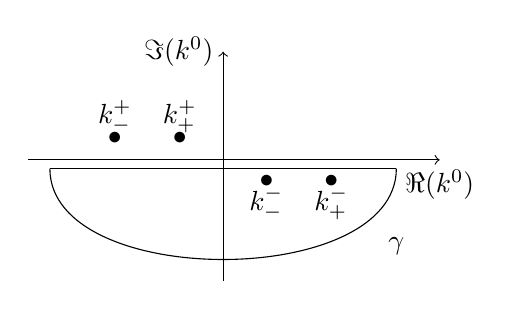
\begin{tikzpicture}[scale=0.55]
    
    % Assi
    \draw[->] (0,-2.8) -- (0,2.5) node[left] {$\Im(k^0)$};
    \draw[->] (-4.5,0) -- (5,0) node[below] {$\Re(k^0)$};
    
    % Piccolo spostamento dell'asse reale (come nel disegno)
    \draw (-4,-0.2) -- (4,-0.2);
    
    % Poli sopra
    \node at (-2.5,1) {$k_-^{+}$};
    \node at (-1.0,1) {$k_+^{+}$};
    
    \draw (-2.5,0.5) node{$\bullet$};
    \draw (-1.0,0.5) node{$\bullet$};
    
    % Poli sotto
    \node at (1.0,-1) {$k_-^{-}$};
    \node at (2.5,-1) {$k_+^{-}$};
    
    \draw (1.0,-0.5) node{$\bullet$};
    \draw (2.5,-0.5) node{$\bullet$};
    
    % Contorno di integrazione
    \draw
    (-4,-0.2)
    .. controls (-4.0,-3.0) and (4.0,-3.0)
    .. (4,-0.2);
    
    % Label gamma
    \node at (4,-2.0) {$\gamma$};
    
    \end{tikzpicture}

    \caption{the poles in the $\selfint{D}(p^2,m^2)$ integrand, the only residue that remains comes from the $k_-^-$ pole.}
    \label{fig: A4 disconiutities in s12 channel}
\end{figure}
\begin{obs}
    We arrive at the same result by applying the rule 
    \begin{equation}
        \begin{split}
            \frac{1}{p_0 - 2E_k + i\smallp} &\longrightarrow -2\pi i\delta[(k \pm p/2)^2 - m^2]\Theta(\pm k^0 + p^0/2) \\
            &\longrightarrow -2\pi i\delta^{(+)}[(k \pm p/2)^2 - m^2].
        \end{split}
    \end{equation}
    This is the Cutkosky rule and can be used to prove the optical theorem.
\end{obs}
We can now continue the analysis of the amplitude since 
\begin{equation}
    \Disc_{p^2}[\amp(p_1p_2 \to p_3p_4)] = -\frac{i\lambda^2}{2}\Disc_{s_{12}}\bigg[\hat{I}_2\bigg(\frac{s_{12}}{m^2},\frac{\mu_R^2}{m^2}\bigg)\bigg] = -\frac{\lambda^2\beta}{16\pi}.
\end{equation}
Since the initial and final states are the same, the optical theorem applies.

\section{Generalised unitarity}
We saw that the discontinuity of a Feynman integral could be computed using the Cutkowsky rule where propagators are replaced with on-shell delta functions
\begin{equation}
    \frac{1}{k^2 - m^2 + i\smallp} \longrightarrow -2\pi i\delta^{(+)}(k^2 - m^2),
\end{equation}
namely
\begin{equation}
    \begin{aligned}
        \Disc_{p^2}[I_2(p^2,m^2)] &= \Disc_{p^2}(\feynmandiagram[inline={([yshift=-0.1cm]current bounding box.center)}, layered layout, horizontal=a to b, scale=0.5, transform shape] { a -- v -- [half left, looseness=1.5] v1 -- [half left, looseness=1.5] v, v1 -- b};) \\
        &\equiv \begin{tikzpicture}[baseline={([yshift=-0.1cm]current bounding box.center)}, scale=0.5, transform shape]
        \begin{feynman}
        
        \vertex (a);
        \vertex [dot, right=0.5cm of a] (v1) {};
        \vertex [dot, right=2cm of v1] (v2) {};
        \vertex [dot, right=0.5cm of v2] (b);
        \vertex [
        below right=1cm and 1.5cm of a] (down) {};
        \vertex [above right=1cm and 1.5cm of a] (up) {};
    
        \diagram* {
          (a) -- (v1),
          (v1) -- [bend right=90] (v2),
          (v2) -- [bend right=90] (v1), (v2) -- (b), (down) -- [ghost] (up)
        };
        \end{feynman}
        \end{tikzpicture} \\
        &= -\int\frac{d^4k}{(2\pi)^4}(2\pi)^2\delta(k^2 - m^2)\delta[(k - p)^2 - m^2] \\
        &= -\frac{\beta}{8\pi}.
    \end{aligned}
\end{equation}
While we lose connection with unitarity, we can replace any propagator in an amplitude with an on-shell $\delta$-function and obtain a ``generalised discontinuity'' of the amplitude. Amplitudes factorise when intermediate propagators go on-shell, for example
\begin{equation}
    \lim_{s_{12} \to 0}(\begin{tikzpicture}[scale=0.7, transform shape, baseline={([yshift=-0.2cm]current bounding box.center)}]
    \begin{feynman}
    
    \vertex (i) {};
    \vertex[right=0.8cm of i, draw, circle, minimum size=0.8cm, inner sep=0pt] (v) {};
    \vertex[above=0.5cm of i] (a) {5};
    \vertex[below=0.5cm of i] (b) {4};
    \vertex[right=0.8cm of v] (f) {};
    \vertex[above=0.5cm of f] (e) {2};
    \vertex[below=0.5cm of f] (g) {3};
    \vertex[above=0.8cm of v] (up) {1};
    
    \diagram* {
        (a) -- (v), (b) -- (v), (v) -- (e), (v) -- (g), (v) -- (up)
    };
    
    \end{feynman}
    \end{tikzpicture}) = \begin{tikzpicture}[scale=0.7, transform shape, baseline={([yshift=-0.1cm]current bounding box.center)}]
    \begin{feynman}
    
    \vertex (i) {};
    \vertex[right=0.8cm of i, draw, circle, minimum size=0.8cm, inner sep=0pt] (v) {};
    \vertex[above=0.5cm of i] (a) {2};
    \vertex[below=0.5cm of i] (b) {1};
    \vertex[right=0.8cm of v] (f) {};
    \vertex[above=0.5cm of f] (e) {};
    \vertex[below=0.5cm of f] (g) {};
    
    \diagram* {
        (a) -- (v), (b) -- (v), (v) -- (f)
    };
    
    \end{feynman}
    \end{tikzpicture}\frac{i}{s_{12}}\begin{tikzpicture}[scale=0.7, transform shape, baseline={([yshift=-0.1cm]current bounding box.center)}]
    \begin{feynman}
    
    \vertex (i) {};
    \vertex[right=0.8cm of i, draw, circle, minimum size=0.8cm, inner sep=0pt] (v) {};
    \vertex[above=0.5cm of i] (a) {};
    \vertex[below=0.5cm of i] (b) {};
    \vertex[right=0.8cm of v] (f) {4};
    \vertex[above=0.5cm of f] (e) {3};
    \vertex[below=0.5cm of f] (g) {5};
    
    \diagram* {
        (i) -- (v), (v) -- (e), (v) -- (g), (v) -- (f)
    };
    
    \end{feynman}
    \end{tikzpicture}.
\end{equation}
This is trivial in scalar theories but in gauge theories relies on the spin sum relations
\begin{gather}
    \slp + m \xrightarrow{p^2 \to m^2} \nsum_su_s\ubar_s, \\
    -g^{\mu\nu} + \frac{p^\mu n^\nu + n^\mu p^\nu}{p \cdot n} \xrightarrow{p^2 \to m^2} \nsum_n\epsilon_n\epsilon_{-n}.
\end{gather}
Hence, when we apply cuts to internal lines we may factorise the integral of an amplitude into products of lower order on-shell amplitudes. The application of multiple cuts to constrain the form of a scattering amplitude is commonly referred to as generalised unitarity.

\subsection{Double-cuts and dispersion relations}
Let's try to use double-cut information to construct the 1-loop $\phi\phi \to \phi\phi$ amplitude. We already saw that 
\begin{equation}
    \Disc_{s_{12}}(\amp_4^{(1)}) = \frac{\lambda^2}{16\pi}\sqrt{1 - \frac{4m^2}{s_{12}}} = \begin{tikzpicture}[scale=0.7, transform shape, baseline={([yshift=-0.1cm]current bounding box.center)}]
    \begin{feynman}
    
    \vertex (i) {};
    \vertex[right=0.8cm of i, draw, circle, minimum size=0.8cm, inner sep=0pt] (v) {0};
    \vertex[above=0.5cm of i] (a) {2};
    \vertex[below=0.5cm of i] (b) {1};
    \vertex[right=0.8cm of v] (f) {};
    \vertex[above=0.5cm of f] (e) {3};
    \vertex[below=0.5cm of f] (g) {4};
    \vertex[above=0.8cm of v] (up) {};
    \vertex[below=0.8cm of v] (down) {};
    
    \diagram* {
        (a) -- (v), (b) -- (v), (v) -- (e), (v) -- (g), (down) -- [ghost] (up)
    };
    
    \end{feynman}
    \end{tikzpicture}.
\end{equation}
The cuts in the other channels, $s_{14}$ and $s_{13}$ are symmetric 
\begin{equation}
    \begin{tikzpicture}[scale=0.7, transform shape, baseline={([yshift=-0.1cm]current bounding box.center)}]
    \begin{feynman}
    
    \vertex (i) {};
    \vertex[right=0.8cm of i, draw, circle, minimum size=0.8cm, inner sep=0pt] (v) {0};
    \vertex[above=0.5cm of i] (a) {1};
    \vertex[below=0.5cm of i] (b) {4};
    \vertex[right=0.8cm of v] (f) {};
    \vertex[above=0.5cm of f] (e) {2};
    \vertex[below=0.5cm of f] (g) {3};
    \vertex[above=0.8cm of v] (up) {};
    \vertex[below=0.8cm of v] (down) {};
    
    \diagram* {
        (a) -- (v), (b) -- (v), (v) -- (e), (v) -- (g), (down) -- [ghost] (up)
    };
    
    \end{feynman}
    \end{tikzpicture} = \frac{\lambda^2}{16\pi}\sqrt{1 - \frac{4m^2}{s_{14}}},\quad \begin{tikzpicture}[scale=0.7, transform shape, baseline={([yshift=-0.1cm]current bounding box.center)}]
    \begin{feynman}
    
    \vertex (i) {};
    \vertex[right=0.8cm of i, draw, circle, minimum size=0.8cm, inner sep=0pt] (v) {0};
    \vertex[above=0.5cm of i] (a) {1};
    \vertex[below=0.5cm of i] (b) {3};
    \vertex[right=0.8cm of v] (f) {};
    \vertex[above=0.5cm of f] (e) {2};
    \vertex[below=0.5cm of f] (g) {4};
    \vertex[above=0.8cm of v] (up) {};
    \vertex[below=0.8cm of v] (down) {};
    
    \diagram* {
        (a) -- (v), (b) -- (v), (v) -- (e), (v) -- (g), (down) -- [ghost] (up)
    };
    
    \end{feynman}
    \end{tikzpicture} = \frac{\lambda^2}{16\pi}\sqrt{1 - \frac{4m^2}{s_{13}}}. 
\end{equation}
To obtain information at the amplitude level we could try to perform dispersion integrals 
\begin{equation}
    f(s) = \frac{1}{2\pi i}\int_\gamma\frac{ds'}{s - s'}\Disc_{s'}[f(s')].
\end{equation}
Since we have a multivariate function this route is more difficult but can be done summing over all the cut contributions. There is however a simpler route if we identify a basis of integrals for the amplitude. The scalar amplitude is trivial, there is no tensor reduction necessary and we can identify from the diagrams by eye 
\begin{equation}
    \amp_4^{(1)} = C_{12}I_2(s_{12},m^2) + C_{23}I_2(s_{23},m^2) + C_{13}I_2(s_{13},m^2),
\end{equation}
from which we use the cut to project out the rational coefficients, namely
\begin{equation}
    \begin{split}
        \Cut_{12}(\amp_4^{(1)}) &= C_{12}\Cut_{12}[I_2(s_{12},m^22)] \\
        \frac{\lambda^2\beta}{16\pi} &= C_{12}\bigg(-\frac{\beta}{8\pi}\bigg) \\
        C_{12} &= -\frac{\lambda^2}{2}.
    \end{split}
\end{equation}
It is possible to show that any 1-loop amplitude can, via tensor reduction, be expressed as linear combination of scalar integrals. If we take external particles to live in four dimensions then the maximum number of independent propagators is four, therefore
\begin{equation}
    \begin{aligned}
        \amp^{(1)}(p_1,\dots,p_n) &= \sum_{B \in box}C_B\feynmandiagram[inline={([yshift=0cm]current bounding box.center)}, scale=0.6, horizontal=v1 to v2] { 
            a -- [edge label'={\tiny B}, pos=0.5] v1, 
            v1 -- v2, 
            v2 -- b, 
            v2 -- v3, 
            v3 -- c, 
            v3 -- v4, 
            v4 -- v1, 
            v4 -- d 
        };[1] + \sum_{T\in triangle}C_T\feynmandiagram[inline={([yshift=0cm]current bounding box.center)}, rotate=-45, horizontal=a to b, scale=0.6] {
        a -- v1 -- v -- v2 -- [edge label={\tiny T}] b, v1 -- v2, v -- c,
        };[1] \\ 
        &+ \sum_{b \in bubble}C_b\feynmandiagram[inline={([yshift=-0.1cm]current bounding box.center)}, layered layout, horizontal=a to b, scale=0.5, transform shape] { a -- v -- [half left, looseness=1.5] v1 -- [half left, looseness=1.5] v, v1 -- b};[1] + R + o(\epsilon),
    \end{aligned}
\end{equation}
where $R$ is a potential rational coefficient coming from
\begin{equation}
    C \cdot I = (C_0 + \epsilon C_1 + \cdots)\bigg(\frac{I_{-1}}{\epsilon} + I_0 + \cdots\bigg) \simeq C_0I + C_1I_{-1}.
\end{equation}
The coefficient $R$ is of UV origin only and is not seen by cuts in four dimension. By using generalised unitarity cuts we can project out the rational coefficients from the factorised loop integrand. Systematic algorithms to proceed iteratively from the maximal cut to determine all coefficients and supplying $D = 4 - 2\epsilon$ information to determine $R$ have been developed. Since there is no integration, this algorithm can be implemented numerically.

\section{Non-Abelian gauge invariance}
We already computed the tree-level amplitude for the $q\qbar gg$ massless scattering
\begin{equation}
\label{eq: tree-level q-qbar-g-g scattering}
    \begin{tikzpicture}[scale=0.7, transform shape, baseline={([yshift=-0.1cm]current bounding box.center)}]
    \begin{feynman}
    
    \vertex (i) {};
    \vertex[right=0.8cm of i, blob, minimum size=0.8cm, inner sep=0pt] (v) {};
    \vertex[above left=0.5cm and 1cm of i, label={[yshift=-0.7cm]\ensuremath{ 2}}] (a) {};
    \vertex[below left=0.5cm and 1cm of i, label=\ensuremath{ 1}] (b) {};
    \vertex[right=0.8cm of v] (f) {};
    \vertex[above right=0.5cm and 1cm of f, label={[yshift=-0.7cm]\ensuremath{ 3}}] (e) {};
    \vertex[below right=0.5cm and 1cm of f, label=\ensuremath{ 4}] (g) {};
    
    \diagram* {
        (a) -- [anti fermion] (v), (b) -- [fermion] (v), (v) -- [gluon] (e), (v) -- [gluon] (g)
    };
    
    \end{feynman}
    \end{tikzpicture} = \begin{tikzpicture}[scale=0.6, transform shape, baseline={([yshift=-0.1cm]current bounding box.center)}]
    \begin{feynman}
    
    \vertex [dot] (a) {};
    \vertex [above left=1cm and 0.7 of a, label={[yshift=-0.7cm]\ensuremath{ 2}}] (v1) {};
    \vertex [below left=1cm and 0.7 of a, label=\ensuremath{ 1}] (v2) {};
    \vertex [dot, right=1.7cm of a] (b) {};
    \vertex [above right=1cm and 0.7 of b, label={[yshift=-0.7cm]\ensuremath{ 3}}] (w1) {};
    \vertex [below right=1cm and 0.7 of b, label=\ensuremath{ 4}] (w2) {};

    \diagram* {
      (v2) -- [fermion] (a) -- [fermion] (v1), (w1) -- [gluon] (b) -- [gluon] (w2),
      (a) -- [gluon] (b)
    };
    \end{feynman}
    \end{tikzpicture} + \begin{tikzpicture}[scale=0.7, transform shape, baseline={([yshift=-0.1cm]current bounding box.center)}]
    \begin{feynman}
    
    \vertex [dot] (a) {};
    \vertex [dot, above=1.3cm of a] (b) {};
    
    \vertex [right=1.2cm of a, label=\ensuremath{ 4}] (v1) {};
    \vertex [left=1.2cm of a, label=\ensuremath{ 1}] (v2) {};
    \vertex [right=1.2cm of b, label={[yshift=-0.7cm]\ensuremath{ 3}}] (w1) {};
    \vertex [left=1.2cm of b, label={[yshift=-0.7cm]\ensuremath{ 2}}] (w2) {};

    \diagram* {
      (a) -- [fermion] (b), (v2) -- [fermion] (a) -- [gluon] (v1), (w2) -- [anti fermion] (b) -- [gluon] (w1)
    };
    \end{feynman}
    \end{tikzpicture} +\begin{tikzpicture}[scale=0.7, transform shape, baseline={([yshift=-0.1cm]current bounding box.center)}]
    \begin{feynman}
    
    \vertex [dot] (a) {};
    \vertex [dot, above=1.3cm of a] (b) {};
    
    \vertex [right=1.2cm of a, label=\ensuremath{ 4}] (v1) {};
    \vertex [left=1.2cm of a, label=\ensuremath{ 1}] (v2) {};
    \vertex [right=1.2cm of b, label={[yshift=-0.7cm]\ensuremath{ 3}}] (w1) {};
    \vertex [left=1.2cm of b, label={[yshift=-0.7cm]\ensuremath{ 2}}] (w2) {};

    \diagram* {
      (a) -- [fermion] (b), (v2) -- [fermion] (a) -- [gluon] (w1), (w2) -- [anti fermion] (b) -- [gluon] (v1)
    };
    \end{feynman}
    \end{tikzpicture}
\end{equation}
and we showed that the Ward identity was satisfied $A^\mu p_{3\mu} = 0$ where $A = A^\mu\epsilon_{3\mu}$. Here we will consider a tensor $M^{\mu\nu}$ where $M^{\mu\nu}\epsilon_{3\mu}\epsilon_{4\nu} = A$, with $|A|^2$ related to $M$ by the spin sum. We write this in a generic gauge as 
\begin{equation}
    \nsum_s\epsilon^\mu_s(p,n)\epsilon^\nu_s(p,n) = -g^{\mu\nu} + P^{\mu\nu}(p,n),
\end{equation}
where
\begin{equation}
    P^{\mu\nu}(p,n) = \frac{p^\mu n^\nu + p^\nu n^\mu}{p \cdot n},\quad n^2 =0.
\end{equation}
Therefore
\begin{equation}
\label{eq: squared amplitude}
    |A|^2 = M^{\mu_3\mu_4}(M^{\nu_3\nu_4})^*[-g_{\mu_3\nu_3} + P_{\mu_3\nu_3}(p_3,n)][-g_{\mu_4\nu_4} + P_{\mu_4\nu_4}(p_4,n)].
\end{equation}
The contributions from diagram 2 and 3 of \eqref{eq: tree-level q-qbar-g-g scattering} to $M^{\mu\nu}$ are 
\begin{equation}
    \begin{split}
        M^{\mu_3\mu_4}_{23} &= -ig_S^2\ubar_1\gamma^{\mu_4}\frac{\slp_{23}}{s_{23}}\gamma^{\mu_3}v_2(t^{a_3}t^{a_4})_{i_2i_1} \\
        &- ig_S^2\ubar_1\gamma^{\mu_3}\frac{\slp_{24}}{s_{24}}\gamma^{\mu_4}v_2(t^{a_3}t^{a_4})_{i_2i_1}.
    \end{split}
\end{equation}
Let's consider the contraction $M^{\mu_3\mu_4}_{23}p_{3\mu}$, we have
\begin{equation}
    \begin{split}
        M^{\mu_3\mu_4}_{23}p_{3\mu} &= -ig_S^2\ubar_1\gamma^{\mu_4}\frac{\slp_{23}}{s_{23}}\slp_3v_2(t^{a_3}t^{a_4})_{i_2i_1} \\
        &- ig_S^2\ubar_1\slp_3\frac{\slp_{24}}{s_{24}}\gamma^{\mu_4}v_2(t^{a_3}t^{a_4})_{i_2i_1} \\
        &= -ig_S^2\ubar_1\gamma^{\mu_4}v_2\comm{t^{a_3}}{t^{a_4}}_{i_2i_1}.
    \end{split}
\end{equation}
The contribution from diagram 1 of \eqref{eq: tree-level q-qbar-g-g scattering} is instead
\begin{equation}
    \begin{split}
        M^{\mu_3\mu_4}_1p_{3\mu_3} &= ig_S^2\ubar_1\gamma^\mu v_2\frac{1}{s_{12}}\comm{t^{a_3}}{t^{a_4}} \\
        &\times [p_3^{\mu_4}(p_3 - p_4)_\mu + g^{\mu_4}_\mu(2p_3 \cdot p_4) + p_{3\mu}(-2p_3 - p_4)^{\mu_4}] \\
        &= ig_S^2\ubar_1\gamma^\mu v_2\frac{1}{s_{12}}[-p_3^{\mu_4}(p_3 + p_4)_\mu + g^{\mu_4\mu}_\mu s_{12} - p_{3\mu}p_4^{\mu_4}]\comm{t^{a_3}}{t^{a_4}}_{i_2i_1} \\
        &= ig_S^2(\ubar_1\gamma^{\mu_4}v_2 - \ubar_1\slp_3v_2p_4^{\mu_4})\comm{t^{a_3}}{t^{a_4}}_{i_2i_1}.
    \end{split}
\end{equation}
Therefore
\begin{equation}
    M^{\mu_3\mu_4}p_{3\mu_3} = ig_S^2\ubar_1\slp_3v_2p_4^{\mu_4}\comm{t^{a_3}}{t^{a_4}}_{i_2i_1}.
\end{equation}
\begin{obs}
    In QED the colour factor is not present so effectively $\comm{t^{a_3}}{t^{a_4}}_{i_2i_1} \to 0$. Also, there are implications for the optical theorem when connecting branch cuts of loop amplitudes to $|A|^2$. 
\end{obs}
The optical theorem states that we must sum over intermediate states, namely
\begin{equation}
    2i\Im{[\amp(q\qbar \to q\qbar)]} = \nsum_k\int d\Phi_k|\amp(q\qbar \to k)|^2.
\end{equation}
In QCD this means we must also consider closed ghost loops and gluon on the left-hand side by
\begin{equation}
\begin{aligned}
    \amp^{(1)}(q\qbar \to q\qbar) &= \feynmandiagram[ 
        inline={([yshift=-0.1cm]current bounding box.center)}, 
        scale=0.7, 
        transform shape, 
        horizontal=v1 to v2
    ] { 
        a -- v1, 
        v1 -- [gluon] v2, 
        v2 -- b, 
        v2 -- v3, 
        v3 -- c, 
        v3 -- [gluon] v4, 
        v4 -- v1, 
        v4 -- d 
    }; + \cdots +
    \feynmandiagram[inline={([yshift=-0.1cm]current bounding box.center)}, horizontal=a to c, scale=0.8, transform shape, rotate=45] { a -- b -- c, b -- [gluon] b1 [dot] -- [gluon, half left, looseness=1.5] v [dot] -- [gluon, half left, looseness=1.5] b1, v -- [gluon] d, d -- e, d -- f}; \\
    &+ \feynmandiagram[inline={([yshift=-0.1cm]current bounding box.center)}, horizontal=a to c, scale=0.8, transform shape, rotate=45] { a -- b -- c, b -- [gluon] b1 [dot] -- [ghost, half left, looseness=1.5] v [dot] -- [ghost, half left, looseness=1.5, with arrow=0.5] b1, v -- [gluon] d, d -- e, d -- f}; + \feynmandiagram[inline={([yshift=-0.1cm]current bounding box.center)}, horizontal=a to c, scale=0.8, transform shape, rotate=45] { a -- b -- c, b -- [gluon] b1 [dot] -- [ghost, half right, looseness=1.5, with arrow=0.5] v [dot] -- [ghost, half right, looseness=1.5] b1, v -- [gluon] d, d -- e, d -- f};.
\end{aligned}
\end{equation}
To see this is all consistent with our computation of $M^{\mu_3\mu_4}$ we may also look at another amplitude 
\begin{equation}
    \begin{aligned}
        \amp_{ghost}(3,4) &= \begin{tikzpicture}[scale=0.6, transform shape, baseline={([yshift=-0.1cm]current bounding box.center)}]
        \begin{feynman}
        
        \vertex [dot] (a) {};
        \vertex [above left=1cm and 0.7 of a, label={[yshift=-0.7cm]\ensuremath{\scriptstyle 3}}] (v1) {};
        \vertex [below left=1cm and 0.7 of a, label=\ensuremath{\scriptstyle 1}] (v2) {};
        \vertex [dot, right=1.7cm of a] (b) {};
        \vertex [above right=1cm and 0.7 of b, label={[yshift=-0.7cm]\ensuremath{\scriptstyle 3}}] (w1) {};
        \vertex [below right=1cm and 0.7 of b, label=\ensuremath{\scriptstyle 4}] (w2) {};
    
        \diagram* {
          (v2) -- [fermion] (a) -- [fermion] (v1), (w1) -- [ghost] (b) -- [ghost] (w2),
          (a) -- [gluon] (b)
        };
        \end{feynman}
        \end{tikzpicture} \\
        &= ig_S^2\ubar_1\gamma^\mu v_2\frac{1}{s_{12}}p_{3\mu}\comm{t^{a_4}}{t^{a_3}}_{i_2i_1} \\
        &= -ig_S^2\ubar_1\slp_3v_2\frac{1}{s_{12}}\comm{t^{a_4}}{t^{a_3}}_{i_2i_1}.
    \end{aligned}
\end{equation}
This very similar to the result obtained for $M^{\mu_3\mu_4}p_{3\mu_3} = p^{\mu_4}_4\amp_{ghost}(3,4)$. Swapping 3 with 4 gives another relation $M^{\mu_3\mu_4}p_{4\mu_4} = p^{\mu_3}_3\amp_{ghost}(4,3)$, that we can use when expanding the tree amplitude squared using equation \eqref{eq: squared amplitude}, namely
\begin{equation}
    \begin{split}
        |A|^2 &= M^{\mu_3\mu_4}(M^{\nu_3\nu_4})^*\bigg(-g_{\mu_3\nu_3} + \frac{p_{3\mu_3}n_{\nu_3} + p_{3\nu_3}n_{\mu_3}}{p_3 \cdot n}\bigg) \\
        &\times\bigg(-g_{\mu_4\nu_4} + \frac{p_{4\mu_4}n_{\nu_4} + p_{4\nu_4}n_{\mu_4}}{p_4 \cdot n}\bigg) \\
        &= \underbrace{|M|^2}_{\substack{squared\,amplitude \\ using\,Feynman \\ gauge\,propagator}} + \underbrace{|\amp_{ghost}(3,4)|^2}_{\substack{ghost\,loop\,in\\ one\,direction}} + \underbrace{|\amp_{ghost}(4,3)|^2}_{\substack{ghost\,loop\,in \\ opposite\,direction}}.
    \end{split}
\end{equation}
So we see that the ghost contributions are essential to maintain unitarity when working in the Feynman gauge. Note that if we work in the light-like axial gauge, where the spin sum matches the Feynman rule for the propagator, unitarity is maintained without needing ghosts. 

\subsection{BRST symmetry}
A complete understanding of non-Abelian gauge invariance, unitarity and the role of ghost fields may be using the formalism of Becchi, Rouet, Stora and Tyutin. The issue is that while the classical QCD Lagrangian (one quark flavour)
\begin{equation}
    \dL^{(QCD)}_{C} = -\frac{1}{4}F^a_{\mu\nu}F^{a\mu\nu} + \psib(i\slD - m)\psi
\end{equation}
is invariant under $SU(n_c)$ rotations, quantisation of the gauge field introduces new elements to the Lagrangian 
\begin{equation}
    \dL^{(QCD)}_{gauge} = -\frac{1}{2\xi}(\p_\mu A^{a\mu})^2,\quad \dL_{ghost}^{(QCD)} = -\cbar^a \p_\mu D^\mu_{ab}c^b,
\end{equation}
for covariant gauge fixing and ghosts respectively. These terms break the invariance of the Lagrangian under $SU(n_c)$ rotations. There is however a hidden symmetry that we can uncover through the addition of an auxiliary scalar field $B^a$. Let's compare two Lagrangians, namely
\begin{align}
    \dL^{(QCD)} &= \dL^{(QCD)}_C + \dL^{(QCD)}_{gauge} + \dL_{ghost}^{(QCD)}, \\
    \begin{split}
        \dL^{(QCD)}_B &= \dL^{(QCD)}_C + \dL^{(QCD)}_{ghost} + \frac{\xi}{2}(B^a)^2 + B^a\p_\mu A^{\mu a} \\
        &\equiv \dL_C^{(QCD)} + \dL^{(QCD)}_{ghost} + \dL^{(QCD)}_{aux}.
    \end{split}
\end{align}
Derivatives of the field $B^a$ do not appear in $\dL^{(QCD)}_{aux}$ hence it is a non-dynamical field. We may integrate this field out of the Lagrangian using a generating function, so
\begin{equation}
    \begin{split}
        \int DB\exp{\bigg(i\int d^4x\,\dL^{(QCD)}_{aux}\bigg)} &= \int DB\exp{\bigg[\frac{i\xi}{2}\int d^4x\,\bigg(B^a + \frac{1}{\xi}\p_\mu A^{a\mu}\bigg)^2} \\
        &\times \int DB\exp{\bigg[-\frac{1}{\xi^2}(\p_\mu A^{a\mu})^2\bigg]} \\
        &= \exp{\bigg[-i\int d^4x\,\frac{1}{2\xi}(\p_\mu A^{a\mu})^2\bigg]} \\
        &\int DB'\exp{\bigg[i\int d^4x\,(B'^{a})^2\bigg]} \\
        &\equiv \norm\exp{\bigg[-i\int d^4x\,\frac{1}{2\xi}(\p_\mu A^{a\mu})^2\bigg]},
    \end{split}
\end{equation}
where the normalization $\norm$ will cancel for any correlation function so we may say $\dL^{(QCD)}_B = \dL^{(QCD)}$ since they produce identical physics. Recall correlation function in a scalar theory 
\begin{equation}
    \mybrakett{0}{T\{\phi_1\cdots\phi_n\}}{0} = \lim_{T \to \infty} \frac{\displaystyle\int D\phi\bigg[\phi_1\cdots\phi_n\exp{\bigg(i\displaystyle\int d^4x\,\dL\bigg)}\bigg]}{\displaystyle\int D\phi\bigg[\exp{\bigg(i\displaystyle\int d^4x\,\dL\bigg)}\bigg]}.
\end{equation}
The Lagrangian $\dL^{(QCD)}_B$ is symmetric under a global transformation written using an anti-commuting Grassmann parameter $\theta$, namely
\begin{gather}
    \delta_\theta A^{a\mu} = \theta D^{ab}_\mu c^b,\quad \delta_\theta\psi = ig_S\theta c^at^a\psi,\quad \delta_\theta c^a = -\frac{g_S}{2}\theta f^{abc}c^bc^c, \\
    \delta_\theta\cbar^a = \theta B^a,\quad \delta_\theta B^a = 0.
\end{gather}
The quantities $\delta A^{a\mu}$ and $\delta\psi$ are equivalent to infinitesimal $SU(n_c)$ rotations through an angle $\theta_{SU}$ such that 
\begin{equation}
    \Theta = \theta^a_{SU}(x)t^a = \theta c^a(x)t^a \equiv\theta_{SU}(x)t^a,\quad \theta_{SU}(x) \equiv \theta c^a(x)
\end{equation}
Recall $SU(n_c)$ transformation led to 
\begin{gather}
    A'_\mu = A_\mu - D_\mu\theta + o(\theta^2),\quad \psi' = \exp{(ig_S\theta)}\psi = (1 + ig_S\theta)\psi + o(\theta^2).
\end{gather}
We have the correct sign since $\theta$ anti-commutates with $c^a$, namely $\theta c^a(x) = -c^a(x)\theta$. We may now show that $\delta_\theta(\dL^{(QCD)}) = \delta_\theta(\dL_B^{(QCD)}) = 0$ by noting that $\delta_\theta(\dL^{(QCD)}_B) = 0$ for $SU(n_c)$ rotations, that 
\begin{equation}
    \begin{split}
        \delta_\theta(\dL^{(QCD)}_B) &= \delta_\theta\bigg[\frac{\xi}{2}(B^a)^2 + B^a\p_\mu A^{a\mu}\bigg] \\
        &= \frac{\xi}{2}\cancelto{0}{\delta_\theta[(B^a)^2]} + \cancelto{0}{\delta_\theta(B^a)}\p_\mu A^{a\mu} + B^a\p_\mu\delta_\theta(A^{a\mu}) \\
        &= B^a\gamma^\mu(\theta D_\mu^{ab}c^b),
    \end{split}
\end{equation}
and that 
\begin{equation}
    \begin{split}
        \delta_\theta(\dL^{(QCD)}_{ghost}) &= \delta_\theta(-\cbar^a\p_\mu D^{\mu ab}A^{\mu c}c^b) \\
        &= -\delta_\theta(\cbar^a)\p_\mu D^{\mu ab}c^b - \cbar^a\p_\mu\delta_\theta(\p^\mu c^a + g_Sf^{abc}A^{\mu c}c^b) \\
        &= -\theta B^a\p_\mu D^{\mu ab}c^b - \cbar^a\p_\mu\p^\mu\bigg(-\frac{1}{2}\theta f^{abc}c^bc^c\bigg) \\
        &-\cbar^a\p_\mu\{g_Sf^{abc}[(\delta_\theta A^{\mu c})c^b + A^{\mu c}\delta_\theta(c^b)]\} \\
        &= -\theta B^a\p_\mu D^{\mu ab}c^b - \cbar^a\p_\mu \p^\mu\bigg(-\frac{1}{2}\theta f^{abc}c^bc^c\bigg) \\
        &-g_Sf^{abc}\cbar^a\p_\mu\bigg[\theta(D^{\mu cd}c^d)c^b + A^{\mu c}\bigg(-\frac{1}{2}g_S\theta f^{bde}c^dc^e\bigg)\bigg] \\
        &= -\theta B^a\p_\mu D^{\mu ab}c^b + g_S\cbar^a\p_\mu \theta f^{abc}\frac{1}{2}\p^\mu(c^bc^c) \\
        &- g_Sf^{abc}\cbar^a\theta\p_\mu\bigg[(\p^\mu c^c)c^b + g_Sf^{cde}A^{\mu e}c^dc^b - \frac{1}{2}g_Sf^{bde}A^{\mu c}c^dc^e\bigg] \\
        &= -\theta B^a \p_\mu D^{\mu ab}c^b \\
        &= -\delta_\theta(\dL^{(QCD)}_{aux}),
    \end{split}
\end{equation}
where in the last step we collected terms at order $o(g_S)$ and $o(g_S^2)$ that cancel thanks to the Jacobi identity. Therefore
\begin{equation}
    \delta_\theta(\dL^{(QCD)}) = 0.
\end{equation}
This global symmetry implies a conserved Noether current $\p_\mu j^\mu_{BRST} = 0$, from which we may also take a conserved charge $\p_0Q_{BRST} = 0$ where
\begin{equation}
    Q_{BRST} = \int d^3x\,j^0_{BRST},
\end{equation}
which commutes with the Hamiltonian, namely $\comm{Q_{BRST}}{\hatH} = 0$. The variation of the gauge field can be written in terms of the BRST charge by
\begin{equation}
    \delta_\theta A^a_\mu = \theta\comm{Q_{BRST}}{A^a_\mu}
\end{equation}
and similarly for other fields, like $B$, $c$, $\cbar$, and $\psi$. We can say this with a simpler notation $\delta_\theta F = \theta QF$.

\subsubsection{Implications of BRST symmetry for unitarity}
A nilpotent operator $Q$ that commutes with the Hamiltonian will divide the Hilbert space $\SH$ into three subspaces:
\begin{enumerate}
    \item $\SH_0$ with states $\ket{\psi_0}$ where $Q\ket{\psi_0} = 0$ and where it doesn't exists a $\ket{\phi} \in \SH$ satisfying $\ket{\psi_0} = Q\ket{\phi}$;
    \item $\SH_1$ with states $\ket{\psi_1}$ where $Q\ket{\psi_1} \neq 0$;
    \item $\SH_2$ with states $\ket{\psi_2}$ where $\ket{\psi_2} = Q\ket{\phi}$ such that $Q\ket{\psi_2} = Q^2\ket{\phi} = 0$.
\end{enumerate}
This defines the BRST cohomology, which it is the first hint of a deep mathematical structure. We see the states of $\SH_2$ are orthogonal, in fact
\begin{equation}
    \mybraket{\psi_2}{\psi_2'} = \mybrakett{\phi}{Q^\dg Q}{\phi} = \mybrakett{\phi}{Q^2}{\phi} = 0,\quad \ket{\psi_2},\ket{\psi_2'} \in \SH_2.
\end{equation}
Moreover, we see the states of $\SH_2$ are orthogonal to those of $\SH_0$, in fact
\begin{equation}
    \mybraket{\psi_2}{\psi_0} = \mybrakett{\psi_2}{Q^\dg}{\psi_0} = \mybrakett{\psi_2}{Q}{\psi_0} = 0,\quad \ket{\psi_2} \in \SH_2,\,\ket{\psi_0} \in \SH_0.
\end{equation}
We can interpret the structure as follows:
\begin{enumerate}
    \item the $\SH_0$ space physical states;
    \item the $\SH_1$ and $\SH_2$ space contain unphysical states, namely ghosts and longitudinal polarisations.
\end{enumerate}
Using the BRST charge and the states of each subspace we may prove the unitarity of the $S$-matrix, namely
\begin{equation}
    \comm{Q_{BRST}}{\hatH} = 0 \Longleftrightarrow \comm{Q}{S} = 0.
\end{equation}
Therefore, for $\ket{\psi_0} \in \SH_0$ we have
\begin{equation}
    0 = \comm{Q}{S}\ket{\psi_0} = (QS - SQ)\ket{\psi_0} = QS\ket{\psi_0}.
\end{equation}
This means that the states $S\ket{\psi_0}$ must be in $\SH_0$ or $\SH_2$ and not in $\SH_1$, thus $S\ket{\psi_0} \in \SH_0 \op \SH_2$. Now consider two physical states $\ket{\psi_0}$ and $\ket{\psi_0'}$ from $\SH_0$, where
\begin{equation}
    \mybraket{\psi_0'}{\psi_0} = \mybrakett{\psi_0'}{S^\dg S}{\psi_0},\quad S^\dg S = \MI.
\end{equation}
We can insert a complete set of states with the relation $\sum_{\psi \in \SH}\ket{\psi}\bra{\psi} = \MI$ obtaining
\begin{equation}
    \begin{split}
        \mybrakett{\psi_0}{S^\dg S}{\psi_0'} = \sum_{\psi \in \SH}\mybrakett{\psi_0'}{S^\dg}{\psi}\mybrakett{\psi}{S}{\psi_0} &= \sum_{\psi_0'' \in \SH_0}\mybrakett{\psi_0'}{S^\dg}{\psi_0''}\mybrakett{\psi_0''}{S}{\psi_0} \\
        &+ \sum_{\psi_1 \in \SH_1}\mybrakett{\psi_0'}{S^\dg}{\psi_1}\cancelto{0}{\mybrakett{\psi_1}{S}{\psi_0}} \\
        &+ \sum_{\psi_2 \in \SH_2}\mybrakett{\psi_0'}{S^\dg}{\psi_2}\cancelto{0}{\mybrakett{\psi_2}{S}{\psi_0}} \\
        &= \sum_{\psi_0'' \in \SH_0}\mybrakett{\psi_0'}{S^\dg}{\psi_0''}\mybrakett{\psi_0''}{S}{\psi_0},
    \end{split}
\end{equation}
where we used the fact that $\SH_1$ is orthogonal to $\SH_0 \op \SH_2$ and that $\SH_2$ is orthogonal to $\SH_1 \op \SH_2$. Thus, the $S$-matrix for the physical states is unitary.

\section{Effective field theories}
We have stated that theories with operators of mass dimension higher than four are not renormalizable in a 4-dimensional spacetime. We may relax this condition if we only require our field theory to apply within a specific energy regime and define an effective field theory. The Fermi theory of the weak interaction is the most famous example
\begin{equation}
\begin{aligned}
    \begin{tikzpicture}[scale=0.6, transform shape, baseline={([yshift=-0.1cm]current bounding box.center)}]
    \begin{feynman}
    
    \vertex [dot] (a) {};
    \vertex [above left=1.2cm and 0.7 of a, label={[yshift=-0.7cm]\ensuremath{u}}] (v1) {};
    \vertex [below left=1.2cm and 0.7 of a, label=\ensuremath{\bar{d}}] (v2) {};
    \vertex [dot, right=1.7cm of a] (b) {};
    \vertex [above right=1.2cm and 0.7 of b, label={[yshift=-0.7cm, xshift=0.1cm]\ensuremath{l^+}}] (w1) {};
    \vertex [below right=1.2cm and 0.7 of b, label=\ensuremath{\nu_l}] (w2) {};

    \diagram* {
      (v2) -- [anti fermion] (a) -- [anti fermion] (v1), (w1) -- [fermion] (b) -- [fermion] (w2),
      (a) -- [boson] (b)
    };
    \end{feynman}
    \end{tikzpicture}  &\xrightarrow{m_W \to \infty} \feynmandiagram[inline={([yshift=-0.1cm]current bounding box.center)}, scale = 0.7, horizontal=a to c] { 
    a [label={[yshift=-0.5cm]\ensuremath{\scriptstyle u}}] -- [fermion] b [dot] -- [fermion] d [label=\ensuremath{\scriptstyle \nu_l}], b -- [anti fermion] c [label={[yshift=-0.5cm]\ensuremath{\scriptstyle l^+}}], b -- [fermion] e [label=\ensuremath{\scriptstyle \bar{d}}]}; \\
    \frac{1}{p^2 - m_W^2} &\xrightarrow{m_W \to \infty} -\frac{1}{m_W^2}\bigg(1 + \frac{p^2}{m_W^2} + \cdots \bigg).
\end{aligned}
\end{equation}
We can use an explicit computation of $gg \to H$ via a top quark loop to illustrate how this can work in practice. The process is loop induced in the Standard Model
\begin{equation}
    \begin{tikzpicture}[scale=0.7, transform shape, baseline={([yshift=-0.1cm]current bounding box.center)}]
    \begin{feynman}
    
    \vertex (i) {};
    \vertex[right=1cm of i, blob, minimum size=0.7cm, inner sep=0pt] (v) {};
    \vertex[above=0.5cm of i] (a) {};
    \vertex[below=0.5cm of i] (b) {};
    \vertex[right=1cm of v] (f) {};
    \vertex[above=0.5cm of f] (e) {};
    \vertex[below=0.5cm of f] (g) {};
    
    \diagram* {
        (a) -- [gluon] (v), (b) -- [gluon] (v), (v) -- [ghost] (f)
    };
    
    \end{feynman}
    \end{tikzpicture} = \begin{tikzpicture}[scale=0.8, transform shape, baseline={([yshift=-0.1cm]current bounding box.center)}]
    \begin{feynman}
    
    \vertex (a) {};
    \vertex [left=1cm of a, draw, circle, minimum size=0.6cm, inner sep=0pt] (v) {};
    \vertex [above left=0.5cm and 1cm of v] (b) {};
    \vertex [below left=0.5cm and 1cm of v] (c) {};
    
    \diagram* {
        (a) -- [ghost] (v),
        (v) -- [gluon] (b),
        (v) -- [gluon] (c),
    };
    
    \end{feynman}
    
    % freccia sulla circonferenza
    \draw[
        postaction={
            decorate,
            decoration={
                markings,
                mark=at position 0.2 with {\arrow{>}}
            }
        }
    ] (v.140) arc (140:-140:0.3cm);
    
    \end{tikzpicture} + \begin{tikzpicture}[scale=0.8, transform shape, baseline={([yshift=-0.1cm]current bounding box.center)}]
    \begin{feynman}
    
    \vertex (a) {};
    \vertex [left=1cm of a, draw, circle, minimum size=0.6cm, inner sep=0pt] (v) {};
    \vertex [above left=0.5cm and 1cm of v] (b) {};
    \vertex [below left=0.5cm and 1cm of v] (c) {};
    
    \diagram* {
        (a) -- [ghost] (v),
        (v) -- [gluon] (b),
        (v) -- [gluon] (c),
    };
    
    \end{feynman}
    
    % freccia sulla circonferenza
    \draw[
        postaction={
            decorate,
            decoration={
                markings,
                mark=at position 0.2 with {\arrow{>}}
            }
        }
    ] (v.-400) arc (-400:400:0.3cm);
    
    \end{tikzpicture} + o(g_S^4y_t,g_S^2y_t^3,g_S^2y_tg_W^2).
\end{equation}
The relevant part of the Standard Model is 
\begin{equation}
    \dL_{SM} = \cdots + y_tH\psib_t\psi_t + \psib_t(i\slD - m_t)\psi_t + \cdots,
\end{equation}
where distinguishing between left and right handed quark fields is not relevant. In the region $\sqrt{s} \ll (m_t,m_H)$ we may use an approximation for $m_t \to \infty$ to have
\begin{equation}
     \underbrace{\dL_{SM}}_{\substack{contains\\\begin{tikzpicture}[scale=0.7, transform shape, baseline={([yshift=-0.1cm]current bounding box.center)}]
    \begin{feynman}
    
    \vertex (a) {};
    \vertex [left=1cm of a, draw, circle, minimum size=0.6cm, inner sep=0pt] (v) {};
    \vertex [above left=0.5cm and 1cm of v] (b) {};
    \vertex [below left=0.5cm and 1cm of v] (c) {};
    
    \diagram* {
        (a) -- [ghost] (v),
        (v) -- [gluon] (b),
        (v) -- [gluon] (c),
    };
    
    \end{feynman}
    
    % freccia sulla circonferenza
    \draw[
        postaction={
            decorate,
            decoration={
                markings,
                mark=at position 0.2 with {\arrow{>}}
            }
        }
    ] (v.140) arc (140:-140:0.3cm);
    
    \end{tikzpicture}}} \xrightarrow{m_t \to \infty} \dL_{SM}^{(no\,top)} + \underbrace{\dL_{eff}}_{\substack{contains\\ \begin{tikzpicture}[scale=0.7, transform shape, baseline={([yshift=-0.1cm]current bounding box.center)}]
    \begin{feynman}
    
    \vertex (a) {};
    \vertex [left=1cm of a, dot] (v) {};
    \vertex [above left=0.5cm and 1cm of v] (b) {};
    \vertex [below left=0.5cm and 1cm of v] (c) {};
    
    \diagram* {
        (a) -- [ghost] (v),
        (v) -- [gluon] (b),
        (v) -- [gluon] (c),
    };
    
    \end{feynman}
    
    \end{tikzpicture}}}.
\end{equation}
Since we have the technology to compute the loop diagram directly we may see how to write $\dL_{eff}$ in terms of a 5-dimensional operator. The two diagrams are symmetric so $\amp(gg \to H) = 2\D$ where
\begin{equation}
    \D \equiv \begin{tikzpicture}[scale=1.5, transform shape, baseline={([yshift=-0.1cm]current bounding box.center)}]
    \begin{feynman}
    
    \vertex (a) {};
    \vertex [left=1cm of a, draw, circle, minimum size=0.6cm, inner sep=0pt] (v) {};
    \vertex [above left=0.8cm and 1cm of v] (b) {};
    \vertex [below left=0.8cm and 1cm of v] (c) {};

    \vertex [dot, minimum size=0.05cm, above left=0.2cm and 0.23cm of v] (q) {};
    \vertex [dot, minimum size=0.05cm, below left=0.2cm and 0.23cm of v] (q1) {};
    \vertex [dot, minimum size=0.05cm, left=0.7cm of a] (q2) {};
    
    \diagram* {
        (a) -- [ghost, reversed momentum={[arrow distance=5pt]\ensuremath{\scriptstyle p_H}}] (v),
        (v) -- [gluon, reversed momentum={[arrow distance=5pt]\ensuremath{\scriptstyle p_2}}] (b),
        (v) -- [gluon, reversed momentum={[arrow distance=5pt]\ensuremath{\scriptstyle p_1}}] (c),

        (q1) -- [bend left=30, momentum={[arrow distance=4pt]\ensuremath{\scriptstyle k}}] (q), (q) -- [bend left=75, momentum={[arrow distance=4pt]\ensuremath{\scriptstyle k + p_2}}] (q2), (q2) -- [bend left=75, momentum={[arrow distance=4pt]\ensuremath{\scriptstyle k - p_1}}] (q1)
    };
    
    \end{feynman}
    
    % freccia sulla circonferenza
    \draw[
        postaction={
            decorate,
            decoration={
                markings,
                mark=at position 0.2 with {\arrow{>}}
            }
        }
    ] (v.140) arc (140:-140:0.3cm);
    
    \end{tikzpicture},
\end{equation}
where $p_H = p_1 + p_2$. Since the process is loop induced, the amplitude must be finite
\begin{equation}
    \D = (-ig_S)^2\bigg(-\frac{iy_t}{\sqrt{2}}\bigg)\tr{t^{a_1}t^{a_2}}\epsilon_{1\mu_1}\epsilon_{2\mu_2}I^{\mu_1\mu_2},
\end{equation}
where the loop integral is 
\begin{equation}
    I^{\mu_1\mu_2} = \int_k \frac{N^{\mu_1\mu_2}(k)}{D_1D_2D_3},
\end{equation}
where $D_1 \equiv D(k,m_t)$, $D_2 \equiv D(k + p_2,m_t)$, and $D_3 \equiv D(k - p,m_t)$, while the numerator instead is 
\begin{equation}
    N^{\mu_1\mu_2}(k) = \tr{[\gamma^{\mu_1}(\slk + m_t)\gamma^{\mu_2}(\slk + \slp_2 +m_t)(\slk - \slp_1 + m_t)]}.
\end{equation}
We will proceed directly to Feynman parameters and then perform tensor reduction. So 
\begin{equation}
    \begin{split}
        \frac{1}{D_1D_2D_3} &= 2\int_0^1d\alpha_1\int_0^{1 - \alpha_1}d\alpha_2\,\frac{1}{[\alpha_1D_2 + \alpha_2D_3 + (1 - \alpha_1 - \alpha_2)D_1]^3} \\
        &\equiv2\int_0^1d\alpha_1\int_0^{1 - \alpha_1}d\alpha_2\,\frac{1}{\hatD(k)},
    \end{split}
\end{equation}
where $\hatD(k) \equiv \alpha_1D_2 + \alpha_2D_3 + (1 - \alpha_1 - \alpha_2)D_1$ can be shown to be 
\begin{equation}
    \hatD(k) = (k + \alpha_1p_2 -\alpha_2p_1)^2 + 2\alpha_1\alpha_2(p_1 \cdot p_2) - m_t^2 + i\smallp.
\end{equation}
We may now proceed to shift the loop momentum and evaluate the trace in the numerator $N^{\mu_1\mu_2}$. After Feynman parametrisation the diagram can be written as 
\begin{equation}
    I^{\mu\nu} = 2\int_k\int_0^1d\alpha_1\int_0^{1 - \alpha_1}d\alpha_2\frac{T^{\mu\nu}(k - \alpha_1p_2 + \alpha_2p_1)}{(k^2 - m_t^2 + \alpha_1\alpha_2m_H^2)^3},
\end{equation}
where 
\begin{equation}
    \epsilon_{1\mu_1}\epsilon_{2\nu}T^{\mu\nu}(k) = 4m_t\bigg[g^{\mu\nu}\bigg(-k^2 - \frac{m_H^2}{2} - m_t^2\bigg) + 4k^\mu k^\nu + p_1^\nu p_2^\mu\bigg]\epsilon_{1\mu}\epsilon_{2\nu}.
\end{equation}
For the tensor reduction in the Feynman parameter space we make use of 
\begin{equation}
    \int_k\frac{k^\mu k^\nu}{(k^2 - \Delta)^n} = \frac{1}{D}g^{\mu\nu}\int_k\frac{k^2}{(k^2 - \Delta)^n},\quad \int_k\frac{k^\mu}{(k^2 - \Delta)^n} = 0,
\end{equation}
after of which we have
\begin{equation}
    \begin{split}
        I^{\mu\nu} &= 2\int_k\int_\alpha\bigg\{g^{\mu\nu}\bigg[\frac{D - 4}{D}k^2 - m_t^2 + m_H^2(1- 2\alpha_1\alpha_2)\bigg] - p_1^\nu p_2^\mu(1 - 4\alpha_1\alpha_2)\bigg\} \\
        &\times\frac{4m_t}{(k^2 - m_t^2 + m_H^2\alpha_1\alpha_2)^3}.
    \end{split}
\end{equation}
The next step is integration over $k$ using the results 
\begin{align}
    \int_k\frac{1}{(k^2 - \Delta)^3} &= \frac{i(4\pi)^\epsilon}{(4\pi)^2}\Gamma(1 + \epsilon)\frac{\Delta^{-1-\epsilon}}{2}, \\
    \int_k\frac{k^2}{(k^2 - \Delta)^3} &= \frac{i(4\pi)^\epsilon}{(4\pi)^2}\Gamma(1 + \epsilon)\bigg(\frac{2 - \epsilon}{\epsilon}\bigg)\Delta^{-\epsilon}.
\end{align}
The $1/\epsilon$ pole in the $k^2$ integral is cancelled by the coefficient $D - 4 = -2\epsilon$ in front so the result is finite as expected. Through Feynman parameter integration one can also show that
\begin{equation}
    F\bigg(\frac{m_H^2}{m_t^2}\bigg) = \int_\alpha\frac{1 - 4\alpha_1\alpha_2}{\bigg(1 - \dfrac{m_H^2}{m_t^2}\alpha_1\alpha_2\bigg)^3}
\end{equation}
is a constant in the limit $1/x \equiv m_t/m_H \to \infty$, namely
\begin{equation}
    \lim_{x \to 0}F(x) = \frac{1}{3} + o(x).
\end{equation}
We have now completed the amplitude computation in the $m_t^2/m_H^2 \to \infty$ limit. Therefore
\begin{equation}
    \amp(gg \to H) \xrightarrow{m_t^2/m_H^2 \to \infty} \frac{\alpha_S}{3\pi v}\delta^{ab}[-g^{\mu\nu}(p_1 \cdot p_2) + p_1^\nu p_2^\mu]\epsilon_{1\mu}\epsilon_{2\nu} + o\bigg(\frac{m_H^2}{m_t^2}\bigg).
\end{equation}
The important feature of this result is  that it has a local structure that can be matched to a local operator
\begin{equation}
    \dL_{eff} = \Wc H\tr{F^{a}_{\mu\nu}F^{a\mu\nu}},
\end{equation}
where $\Wc$ is known as a Wilson coefficient. From this Lagrangian we find the Feynman rule 
\begin{equation}
    \begin{tikzpicture}[scale=1.2, transform shape, baseline={([yshift=-0.1cm]current bounding box.center)}]
    \begin{feynman}
    
    \vertex (i) {};
    \vertex[right=0.8cm of i, crossed dot, minimum size=0.2cm] (v) {};
    \vertex[above=0.5cm of i] (a) {\ensuremath{\scriptstyle2}};
    \vertex[below=0.5cm of i] (b) {\ensuremath{\scriptstyle 1}};
    \vertex[right=0.8cm of v] (f) {\ensuremath{\scriptstyle 3}};
    \vertex[above=0.5cm of f] (e) {};
    \vertex[below=0.5cm of f] (g) {};
    
    \diagram* {
        (a) -- [gluon] (v), (b) -- [gluon] (v), (v) -- [ghost] (f)
    };
    
    \end{feynman}
    \end{tikzpicture} = i\Wc[-g^{\mu_1\mu_2}(p_1 \cdot p_2) + p_1^{\mu_1}p_2^{\mu_2}]
\end{equation}
so matching with the result for $\amp(gg \to H)$ is straightforward 
\begin{center}
    \begin{tikzpicture}
    
        % Nodo in alto a sinistra
        \node at (0,2) {$\dL_{\rm SM}$};
        % Nodo in basso a sinistra
        \node at (0,0) {$A^{(0)}(gg \to H)$};
        % Nodo in alto a destra
        \node at (6,2)
        {$\dL_{SM}^{(no\ top)} + \dL_{eff}$};
        % Nodo in basso a destra
        \node at (6,0)
        {$A_{eff}^{(0)}(gg \to H)
        +  o\bigg(\dfrac{m_H^2}{m_t^2}\bigg)$};
        
        % Freccia verticale sinistra
        \draw[->] (0,1.6) -- (0,0.4);
        % Freccia verticale destra
        \draw[->] (6,1.6) -- (6,0.4);
        % Freccia orizzontale
        \draw[->] (1.3,0) -- (3.7,0);
        % Freccia orizzontale
        \draw[->] (0.5,2) -- (4.5,2);
        
        % Etichetta sopra la freccia
        \node at (2.5,0.2) {$m_t \to \infty$};
        % Etichetta sopra la freccia
        \node at (2.5,2.2) {$m_t \to \infty$};
    
    \end{tikzpicture}.
\end{center}
In general we may construct the set of higher dimension operators satisfying symmetry constraints 
\begin{equation}
    \dL_{eff} = \dL_0 + \sum_{k=1}^\infty\nsum_m\frac{\Wc_m^{(k + 4)}}{\Lambda^k}O_m^{(k + 4)},
\end{equation}
where $\Wc^{(D)}$ are Wilson coefficient of mass dimension $D$ operators $O_m^{(D)}$. The sum over the elements $m$ must be done carefully using a basis of independent operators which accounts for field redefinitions, integration-by-parts identities and equations of motion. Independent operator basis may be quite large; in fact, for the Standard Model with general flavour structure, we easily reach over 2000 operators. 